\documentclass[a4paper, 12pt, slovene]{article}
\usepackage[slovene]{babel}
\usepackage[utf8]{inputenc}
\usepackage{lmodern}
\usepackage[T1]{fontenc}
\usepackage{graphicx}
\usepackage{caption}
\captionsetup{font=footnotesize}
\usepackage{fullpage}
\usepackage{enumitem}
\usepackage{array}
\usepackage{wrapfig}
\usepackage{multirow}
\usepackage{tabularx}
\usepackage{amsmath}
\usepackage{subcaption}
\newcommand*\diff{\mathop{}\!\mathrm{d}}
\newcommand*\Diff[1]{\mathop{}\!\mathrm{d^#1}}
\newcommand*\difft{\mathop{}\!\ddot{ }}
\usepackage{float}
\usepackage{mathrsfs}

\newcommand{\Ai}{\mathrm{Ai}}
\newcommand{\Bi}{\mathrm{Bi}}

\renewcommand{\Re}{\mathop{\rm Re}\nolimits}
\renewcommand{\Im}{\mathop{\rm Im}\nolimits}
\newcommand{\Tr}{\mathop{\rm Tr}\nolimits}
\newcommand{\diag}{\mathop{\rm diag}\nolimits}
\newcommand{\dd}{\,\mathrm{d}}
\newcommand{\ddd}{\mathrm{d}}
\newcommand{\ii}{\mathrm{i}}
\newcommand{\lag}{\mathcal{L}\!}
\newcommand{\ham}{\mathcal{H}\!}
\newcommand{\four}[1]{\mathcal{F}\!\left(#1\right)}
\newcommand{\bigO}[1]{\mathcal{O}\!\left(#1\right)}
\newcommand{\sh}{\mathop{\rm sinh}\nolimits}
\newcommand{\ch}{\mathop{\rm cosh}\nolimits}
\renewcommand{\th}{\mathop{\rm tanh}\nolimits}
\newcommand{\erf}{\mathop{\rm erf}\nolimits}
\newcommand{\erfc}{\mathop{\rm erfc}\nolimits}
\newcommand{\sinc}{\mathop{\rm sinc}\nolimits}
\newcommand{\rect}{\mathop{\rm rect}\nolimits}
\newcommand{\ee}[1]{\cdot 10^{#1}}
\newcommand{\inv}[1]{\left(#1\right)^{-1}}
\newcommand{\invf}[1]{\frac{1}{#1}}
\newcommand{\sqr}[1]{\left(#1\right)^2}
\newcommand{\half}{\frac{1}{2}}
\newcommand{\thalf}{\tfrac{1}{2}}
\newcommand{\pd}{\partial}
\newcommand{\Dd}[3][{}]{\frac{\ddd^{#1} #2}{\ddd #3^{#1}}}
\newcommand{\Pd}[3][{}]{\frac{\pd^{#1} #2}{\pd #3^{#1}}}
\newcommand{\avg}[1]{\left\langle#1\right\rangle}
\newcommand{\norm}[1]{\left\Vert #1 \right\Vert}
\newcommand{\braket}[2]{\left\langle #1 \vert#2 \right\rangle}
\newcommand{\obraket}[3]{\left\langle #1 \vert #2 \vert #3 \right \rangle}
\newcommand{\hex}[1]{\texttt{0x#1}}

\renewcommand{\iint}{\mathop{\int\mkern-13mu\int}}
\renewcommand{\iiint}{\mathop{\int\mkern-13mu\int\mkern-13mu\int}}
\newcommand{\oiint}{\mathop{{\int\mkern-15mu\int}\mkern-21mu\raisebox{0.3ex}{$\bigcirc$}}}

\newcommand{\wunderbrace}[2]{\vphantom{#1}\smash{\underbrace{#1}_{#2}}}

\renewcommand{\vec}[1]{\overset{\smash{\hbox{\raise -0.42ex\hbox{$\scriptscriptstyle\rightharpoonup$}}}}{#1}}
\newcommand{\bec}[1]{\mathbf{#1}}




\begin{document}

\begin{titlepage}
\title{\textsc{Airyjevi funkciji} \\[1ex] \large Prva naloga pri predmetu Matematično-fizikalni praktikum}
\author{Gašper Lotrič, 28191019}
\date{14. oktober 2021}

\maketitle
\end{titlepage}

\tableofcontents
\pagebreak


\section{Naloga}
Z uporabo kombinacije Maclaurinove vrste in asimptotskega razvoja poišči čim učinkovitejši postopek za izračun vrednosti Airyjevih funkcij $\Ai$ in $\Bi$ na vsej realni osi z absolutno napako, manjšo od $10^{-10}$. Enako naredi tudi z relativno napako in ugotovi, ali je tudi pri le-tej dosegljiva natančnost, manjša od $10^{-10}$. Pri oceni napak si pomagaj s programi, ki znajo računati s poljubno natančnostjo, na primer z \textsc{Mathematico} in ali paketi \textsc{Mpmath} in \textsc{Decimal} v programskem jeziku \textsc{Python}.

\section{Uvod}
Airyjevi funkciji se v fiziki uporabljata predvsem v optiki in kvantni mehaniki. Definiramo ju kot rešitvi enačbe
\begin{equation}
y''(x)-xy(x) = 0
\end{equation}
in sta predstavljivi v integralski obliki
\begin{equation*}
  \Ai(x) = \frac{1}{\pi} \int_0^\infty \cos (t^3/3 + x t) \dd t \>,\quad
  \Bi(x) = \frac{1}{\pi} \int_0^\infty \left[ \mathrm{e}^{-t^3/3 + x t}
  + \sin (t^3/3 + x t) \right] \dd t \>.
\end{equation*}
Za majhne $x$ ju lahko razvijemo v Maclaurinove vrste, za velike vrednosti $x$ pa jih lahko obravnavamo z asimptotskimi vrstami. \par\vspace{5mm}

Nalogo sem reševal v programskem jeziku \textsc{Python} in uporabljal knjižnice \textsc{Numpy, Scipy, Matplotlib} in \textsc{Math}. Za referenčne vrednosti $\Ai$ in $\Bi$ sem vzel vrednosti izračunane z \textsl{scipy.special.airy}. Natančno shranjevanje števil v \textsc{Pythonu} sem dosegel s paketom \textsc{Decimal}.


\section{Numerično računanje vrst}
Airyjevi funkciji bom aproksimiral z dvema različnima vrstama: Maclaurinovo in asimptotsko. V tem poglavju bom predstavil računske postopke, ki sem jih uporabil. Rešitev, ki jo dobimo z razvojem po vrstah bo imela željeno vrednost po celi realni osi, razen za $\Bi(x)$ pri velikih pozitivnih številih. Pri računanju vrste se je pametno izogniti računanja gamma funkcije in fakultete za vsak člen.

\subsection{Maclaurinova vrsta}
Funkciji $f$ in $g$ za izračun Maclaurinove vrste sem zapisal v rekurzivni obliki.
\begin{equation}
f_{k+1} = f_k \frac{x^3(1-\frac{2}{3k})}{(3k-1)(3k-2)} \qquad f_0 = \frac{1}{\Gamma(1/3)}
\end{equation}
\begin{equation}
g_{k+1} = g_k \frac{x^3(1-\frac{1}{3k})}{(3k+1)(3k-1)} \qquad g_0 = \frac{x}{\Gamma(1/3)}
\end{equation}
Iz funkcij $f_k$ in $g_k$ bom sestavil $\Ai_k(x)$ in $\Bi_k(x)$ in nato te člene seštel. Smiselno jih je sešteveti od najmanjšega do največjega, saj se tako izognemo numeričnim težavam. Temu se nisem posebaj posvečal. Med seštevanjem sem preverjal velikost najmanjšega člena in pri dovolj natančni vrednosti ($10^{-10}$) prenehal z računanjem. \par\vspace{5mm}

Vrednosti $\Ai$ in $\Bi$ ter njuna odstopanja od pravih vrednosti po sem narisal na sliki \ref{fig-maclaurin}.

\begin{figure}[H]
\centering
\begin{subfigure}{0.49\textwidth}
	\centering
	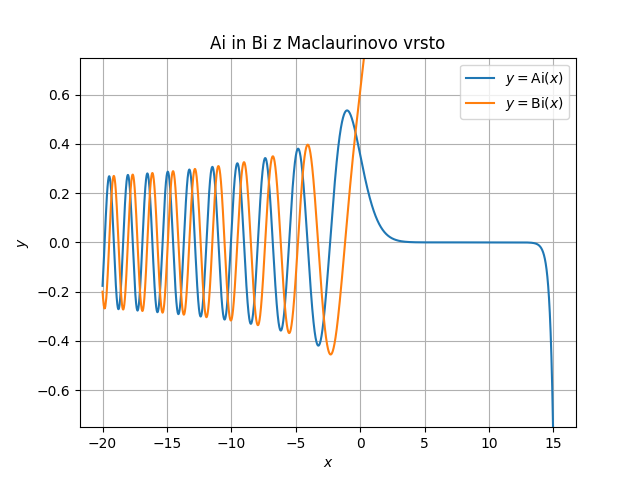
\includegraphics[width=0.95\textwidth]{grafi/maclaurinova.png}
	\caption{Airijevi funkciji z Maclaurinovo vrsto.}
	\label{fig-mcl}
\end{subfigure}%
\begin{subfigure}{0.49\textwidth}
	\centering
	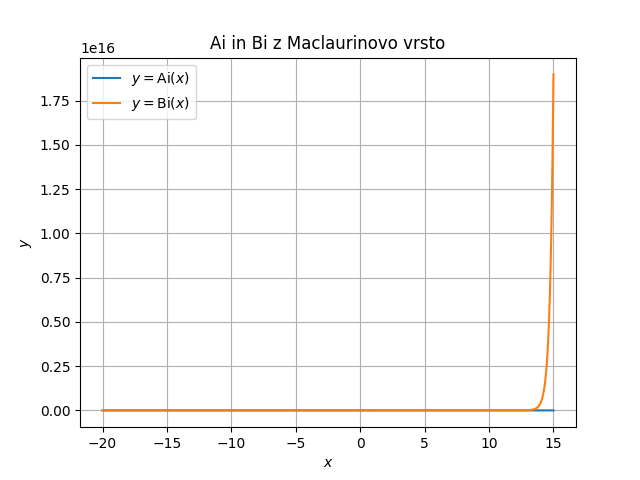
\includegraphics[width=0.95\textwidth]{grafi/maclaurin_velike.png}
	\caption{Maclaurinove vrste za velike vrednosti.}
	\label{fig-mclbig}
\end{subfigure}
\begin{subfigure}{0.49\textwidth}
	\centering
	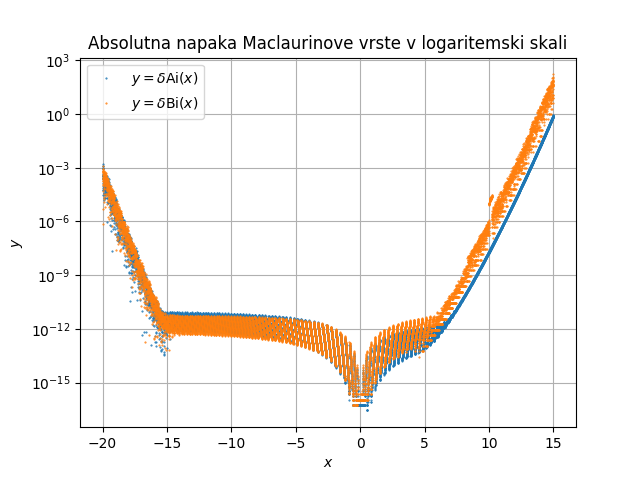
\includegraphics[width=0.95\textwidth]{grafi/maclaurin_abs_err.png}
	\caption{Absolutni napaki Maclaurinovih vrst v logaritemski skali.}
	\label{fig-mcl-abserr-log}
\end{subfigure}
\begin{subfigure}{0.49\textwidth}
	\centering
	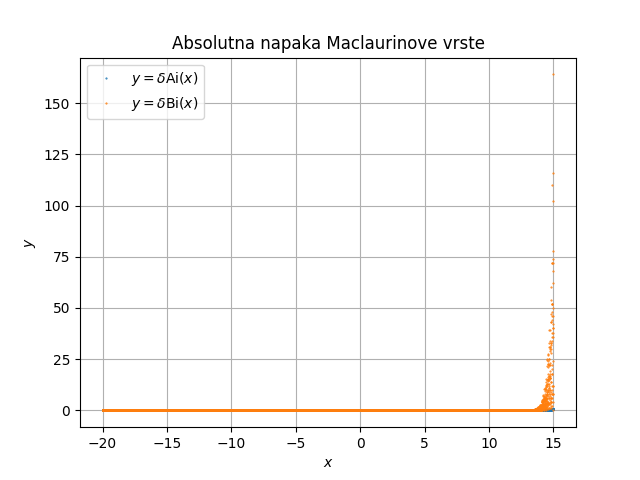
\includegraphics[width=0.95\textwidth]{grafi/maclaurin_abs_err_noscale.png}
	\caption{Absolutni napaki Maclaurinovih vrst.}
	\label{fig-mcl-abserr}
\end{subfigure}
\begin{subfigure}{0.49\textwidth}
	\centering
	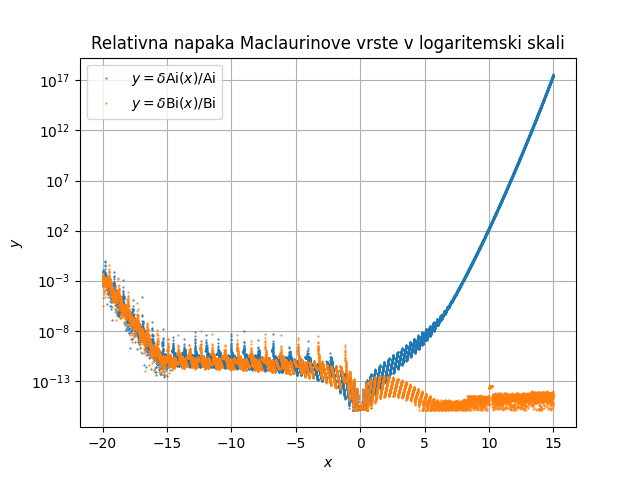
\includegraphics[width=0.95\textwidth]{grafi/maclaurin_rel_err.png}
	\caption{Relativni napaki Maclaurinovih vrst v logaritemski skali.}
	\label{fig-mcl-relerr-log}
\end{subfigure}
\begin{subfigure}{0.49\textwidth}
	\centering
	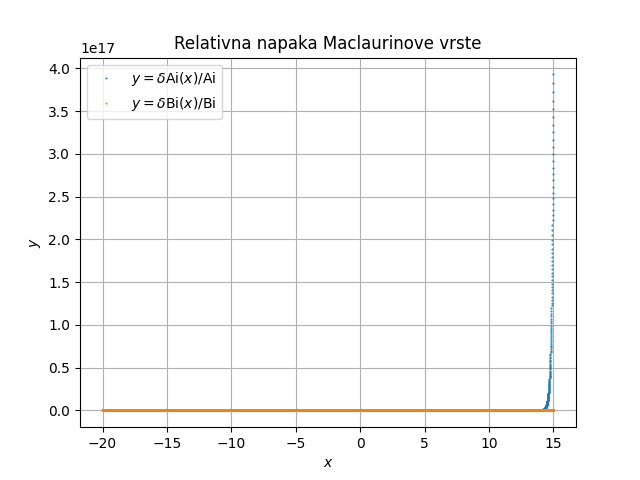
\includegraphics[width=0.95\textwidth]{grafi/maclaurin_rel_err_noscale.png}
	\caption{Relativni napaki Maclaurinovih vrst.}
	\label{fig-mcl-relerr}
\end{subfigure}

\caption{Airyjevi funkciji $\Ai$ in $\Bi$ izračunani z Maclaurinovo vrsto.}
\label{fig-maclaurin}
\end{figure}

Absolutna napaka Maclaurinovih vrst za obe Airyjevi funkciji na intervalu $x\approx[-15, 5]$ ostane celo pod $10^{-11}$, pri večjih pozitivnih in negativnih $x$ z večjo absolutno vrednostjo pa absolutno natančnost hitro izgubljamo (slika \ref{fig-mcl-abserr-log}). \par\vspace{5mm}

Relativna odstopanja Maclaurinove vrste za $\Ai$ se na negativnem delu osi $x$ obnašajo podobno kot absolutna, na pozitivnem delu pa hitro naraščajo (modra krivulja na sliki \ref{fig-mcl-relerr-log}). To se zgodi, ker absolutno natančnost pada, vrednost $\Ai$ pa ostaja majhna. Relativna napaka $\Bi$ pa je zaradi naraščanja funkcije ostala dovolj nizka.


\subsection{Asimptotska vrsta}
Za absolutno velike $|x|$ pa uporabimo aproksimacijo z asimptotskimi vrstami. Ta problem sem obravnaval podobno kot v prejšnjem razdelku. Asimptotske vrste za Airyjevi funkciji se razlikujejo za pozitivne in negativne velike $|x|$. Pri izračunu uporabimo asimptotske vrste:
\begin{equation*}
  L(z) \sim \sum_{s=0}^\infty \frac{u_s}{z^s}\>,\qquad
  P(z) \sim \sum_{s=0}^\infty (-1)^s \frac{u_{2s}}{z^{2 s}}\>,\qquad
  Q(z) \sim \sum_{s=0}^\infty (-1)^s \frac{u_{2s+1}}{z^{2 s+1}}\>,
\end{equation*}
Vrste $L$, $P$, in $Q$ sem zapisal rekurzivno, da sem se spet izognil računanju gamma funkcij in fakultet. S pomočjo treh predfaktorjev sem jih preoblikoval v
\begin{equation}
L_{j+1} = L_j \frac{(3j-\frac{1}{2})(3j-\frac{3}{2})(3j-\frac{5}{2})}{54\xi j (j-\frac{1}{2})} \qquad L_0 = 1
\end{equation}
\begin{equation}
P_{j+1} = P_j(-1)\frac{(6j-\frac{1}{2})(6j-\frac{3}{2})\;...\;(6j-\frac{11}{2})}{54^2\cdot 2j(2j-1)(2j-\frac{1}{2})(2j-\frac{3}{2})\xi^2} \qquad P_0 = 1
\end{equation}
\begin{equation}
Q_{j+1} = Q_j(-1)\frac{(6j+\frac{5}{2})(6j+\frac{3}{2})\;...\;(6j-\frac{5}{2})}{54^2\cdot 2j(2j+1)(2j-\frac{1}{2})(2j+\frac{1}{2})\xi^2} \qquad Q_0 = \frac{(2+\frac{1}{2})(1+\frac{1}{2})}{54\xi}
\end{equation}
Pri čemer je $\xi=\frac{2}{3} |x|^{3/2}$. \par\vspace{5mm}

V okolici izhodišča se je pojavil zanimiv problem; zaustavitveni pogoj je odpovedal in vrednosti faktorjev $L_j$, $P_j$ in $Q_j$ so narasle preko vseh meja. To pomeni, da po nekem členu v asimptostki vrsti vsaj blizu izhodišča členi naraščajo! Zato sem morel zaustavitveni pogoj spremeniti, da se računanje zaustavi, ko se faktorji začnejo povečevati. S takim načinom računanja pa ni nujno, da povsod dosegam željeno absolutno natančnost $10^{-10}$. \par\vspace{5mm}

Obnašanje asimptotskih vrst in njihovih napak sem narisal na sliki \ref{fig-asimptotske}.

\begin{figure}[H]
\centering
\begin{subfigure}{0.49\textwidth}
	\centering
	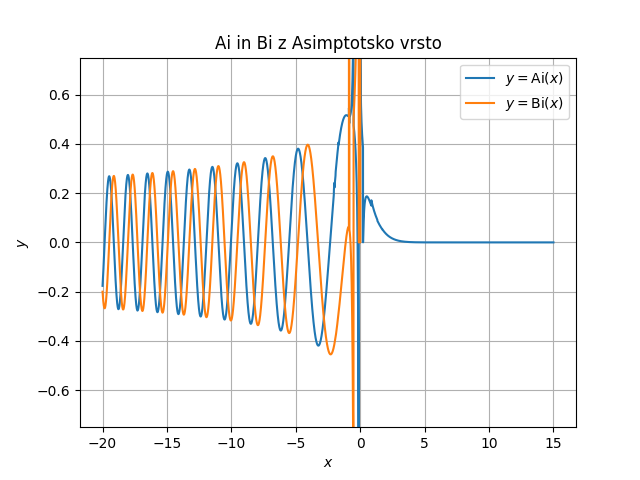
\includegraphics[width=0.95\textwidth]{grafi/asimptotska.png}
	\caption{Airijevi funkciji z Asimptotično vrsto.}
	\label{fig-asi}
\end{subfigure}%
\begin{subfigure}{0.49\textwidth}
	\centering
	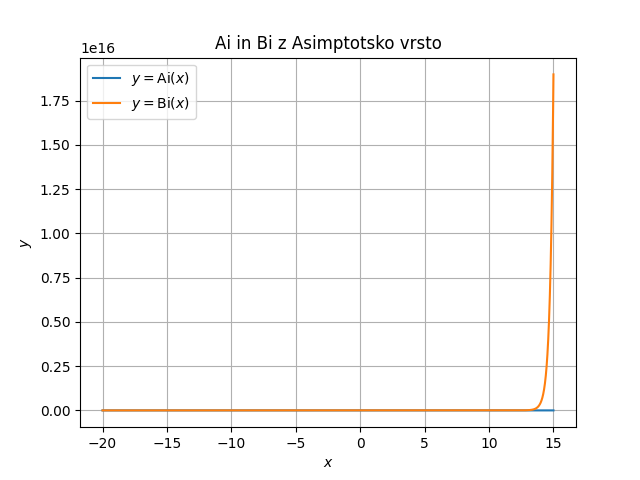
\includegraphics[width=0.95\textwidth]{grafi/asimptotska_velike.png}
	\caption{Asimtotski vrsti za velike vrednosti.}
	\label{fig-asibig}
\end{subfigure}
\begin{subfigure}{0.49\textwidth}
	\centering
	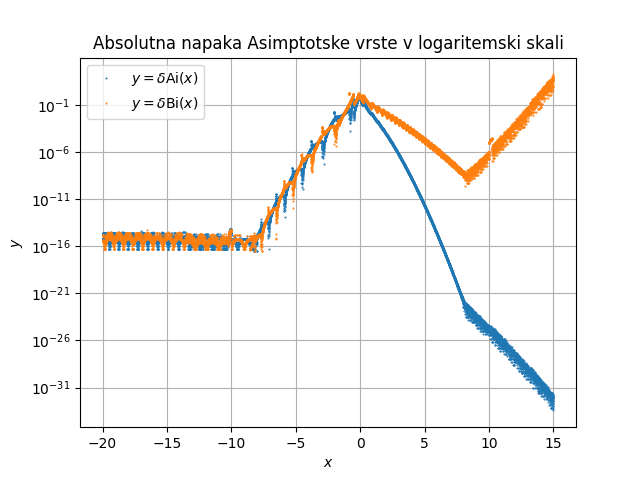
\includegraphics[width=0.95\textwidth]{grafi/asimptotska_abs_err.png}
	\caption{Absolutni napaki asimptotskih vrst v logaritemski skali.}
	\label{fig-asi-abserr-log}
\end{subfigure}
\begin{subfigure}{0.49\textwidth}
	\centering
	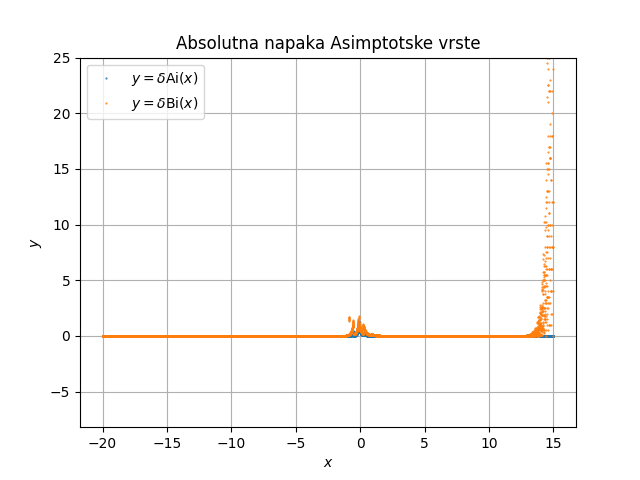
\includegraphics[width=0.95\textwidth]{grafi/asimptotska_abs_err_noscale.png}
	\caption{Absolutni napaki asimptotskih vrst.}
	\label{fig-asi-abserr}
\end{subfigure}
\begin{subfigure}{0.49\textwidth}
	\centering
	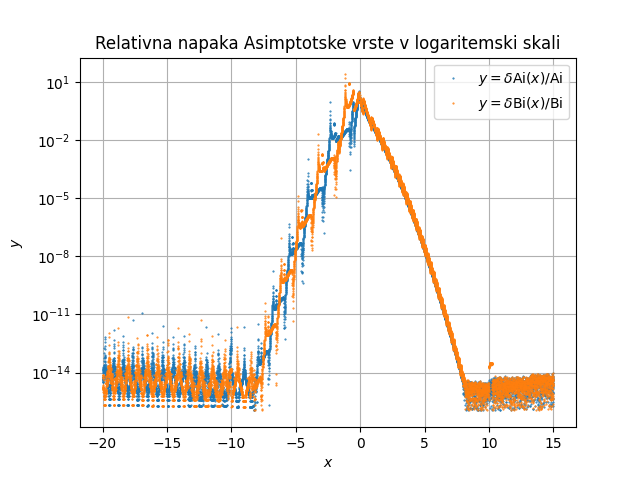
\includegraphics[width=0.95\textwidth]{grafi/asimptotska_rel_err.png}
	\caption{Relativni napaki asimptotskih vrst v logaritemski skali.}
	\label{fig-asi-relerr-log}
\end{subfigure}
\begin{subfigure}{0.49\textwidth}
	\centering
	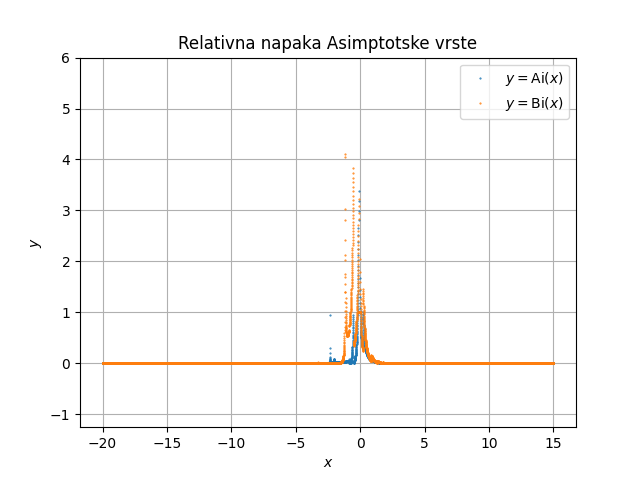
\includegraphics[width=0.95\textwidth]{grafi/asimptotska_rel_err_noscale.png}
	\caption{Relativni napaki asimptotskih vrst.}
	\label{fig-asi-relerr}
\end{subfigure}

\caption{Airyjevi funkciji $\Ai$ in $\Bi$ izračunani z asimptotskimi vrstami.}
\label{fig-asimptotske}
\end{figure}

Zahtevano relativno napako od prave vrednsti asimptotska vrsta za $\Ai$ dosega povsod, razen na intervalu $x\approx[-5, 5]$ (slika \ref{fig-asi-abserr-log}, modra krivulja), kjer ta razvoj ni učinkovit. Podobno veja tudi za relativno napako $\Ai$ (modra krivulja na sliki \ref{fig-asi-relerr-log}). \par\vspace{5mm}

Asimptotska vsta funkcije $\Bi$ pa je malo bolj problematična, saj absolutna napaka pri poziztivnih vrednostih ne pride več nazaj na zahtevanih $10^{-10}$ (oranžna krivulja na sliki \ref{fig-asi-abserr-log}). Ker pa na tem območju funkcija $\Bi$ blazno hitro narašča in relativna napaka ostaja majhna (slika \ref{fig-asi-relerr-log}, oranžna krivuja), je ta rezultat sprejemljiv.


\subsection{Kombinacija vrst}
Maclaurinova vrsta najbolje deluje okrog izhodišča, asimptotski pa za absolutno večje $x$. Zato najboljši približek pravih vrednosti dobimo, če obe vrsti zlepimo. Za absolutno velike negativne $x$ uporabimo negativni asimptotski vrsti, za vrednosti $x$ okoli izhodišča Maclaurinovi vrsti in za velike pozitivne $x$ pozitivni asmiptotski vrsti.\par\vspace{5mm}

Za te mejne vrednosti $x$ sem se odločil na podlagi napak iz prejšnjih dveh poglavij. Maclaurinovo vrsto za $\Ai$ sem uporabljal na intervalu $x = [-6.6, 5.2)$, za $\Bi$ pa na $x = [-6.6, 8.4)$.

\begin{figure}[H]
\centering
\begin{subfigure}{0.49\textwidth}
	\centering
	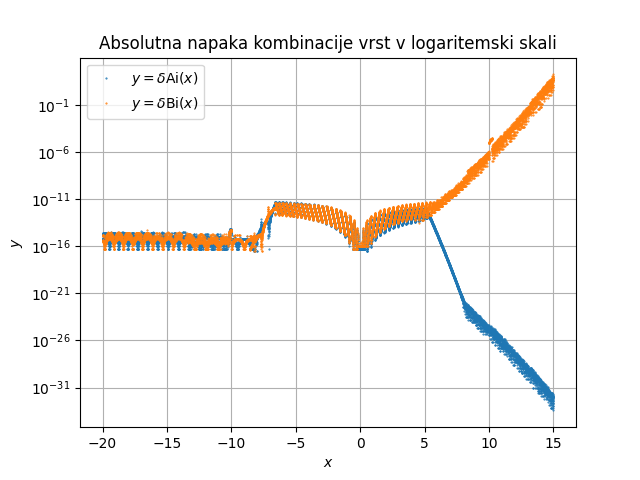
\includegraphics[width=0.95\textwidth]{grafi/kombinacija_abs_err.png}
	\caption{Absolutna napaka kombinacije vrst v logaritemski skali.}
	\label{fig-kom-abserr}
\end{subfigure}%
\begin{subfigure}{0.49\textwidth}
	\centering
	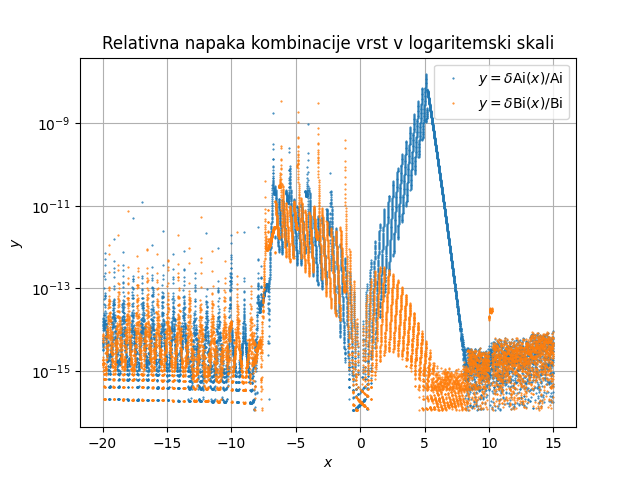
\includegraphics[width=0.95\textwidth]{grafi/kombinacija_rel_err.png}
	\caption{Relativna napaka kombinacije vrst v logaritemski skali.}
	\label{fig-kom-relerr}
\end{subfigure}
\caption{Airyjevi funkciji $\Ai$ in $\Bi$ izračunani s kombinacijo Maclaurinove in asimptotskih vrst.}
\label{fig-kombinacija}
\end{figure}
Absolutna napaka funkcije $\Ai$ stalno manjša od $10^{-11}$, za funkcijo $\Bi$, pa asbolutna napaka po $x\approx 6$ naraste nad $10^{-10}$. \par\vspace{5mm}

Pri računanju relativne napake Airyjeve funkcije $\Ai$ pa sem naletel na nenatančnosti pri na intervalu $x \approx (3, 6)$. tam Maclaurentova vrsta začne zgubljati natančnost, asimptotska pa še ni dovolj točna. Največjo napako sem dobil pri $x = 5.2$, kjer je narasla kar do $1.5\cdot10^{-8}$. Za razliko pa relativna napaka funkcije $\Bi$ ostaja v mejah in ne povzroča preglavic.


\section{Zaključek}
Pametna uporaba matematičnih operacij in konstantna skrb za računalnikovo natančnost sta bila glavna problema te naloge. \par\vspace{5mm}

Pri izračuunu vrst sem dosegel željeno natančnost v vseh primerih, razen pri večjih vrednostih $\Bi(x)$, kjer funkcija ekstremno hitro narašča, absolutna napaka ni dosegla zahtevane. Zadovoljil pa sem z dovolj majhno relativno napako. Probleme mi je povzročala tudi relativna napaka razvojev $\Ai(x)$, saj na nekem intervalu ne Mclaurentova niti asimptotska vrsta nita dosegli željene natančnosti.



\end{document}
